% !TEX encoding = UTF-8 Unicode

\documentclass{standalone}

% packages
\usepackage{float}
\usepackage{tabu}
\usepackage{booktabs}
\usepackage{graphicx}
\usepackage{caption}
\usepackage[export]{adjustbox}
\usepackage[utf8]{inputenc}
%\usepackage[active,pdftex,tightpage]{preview}
\usepackage{newtxtext,newtxmath}
\usepackage[percent]{overpic}

\begin{document}

%\sf
\scriptsize
\centering 

% before and after
\begin{tabular}{m{0.5\textwidth} m{0.5\textwidth}}
%
\multicolumn{1}{c}
{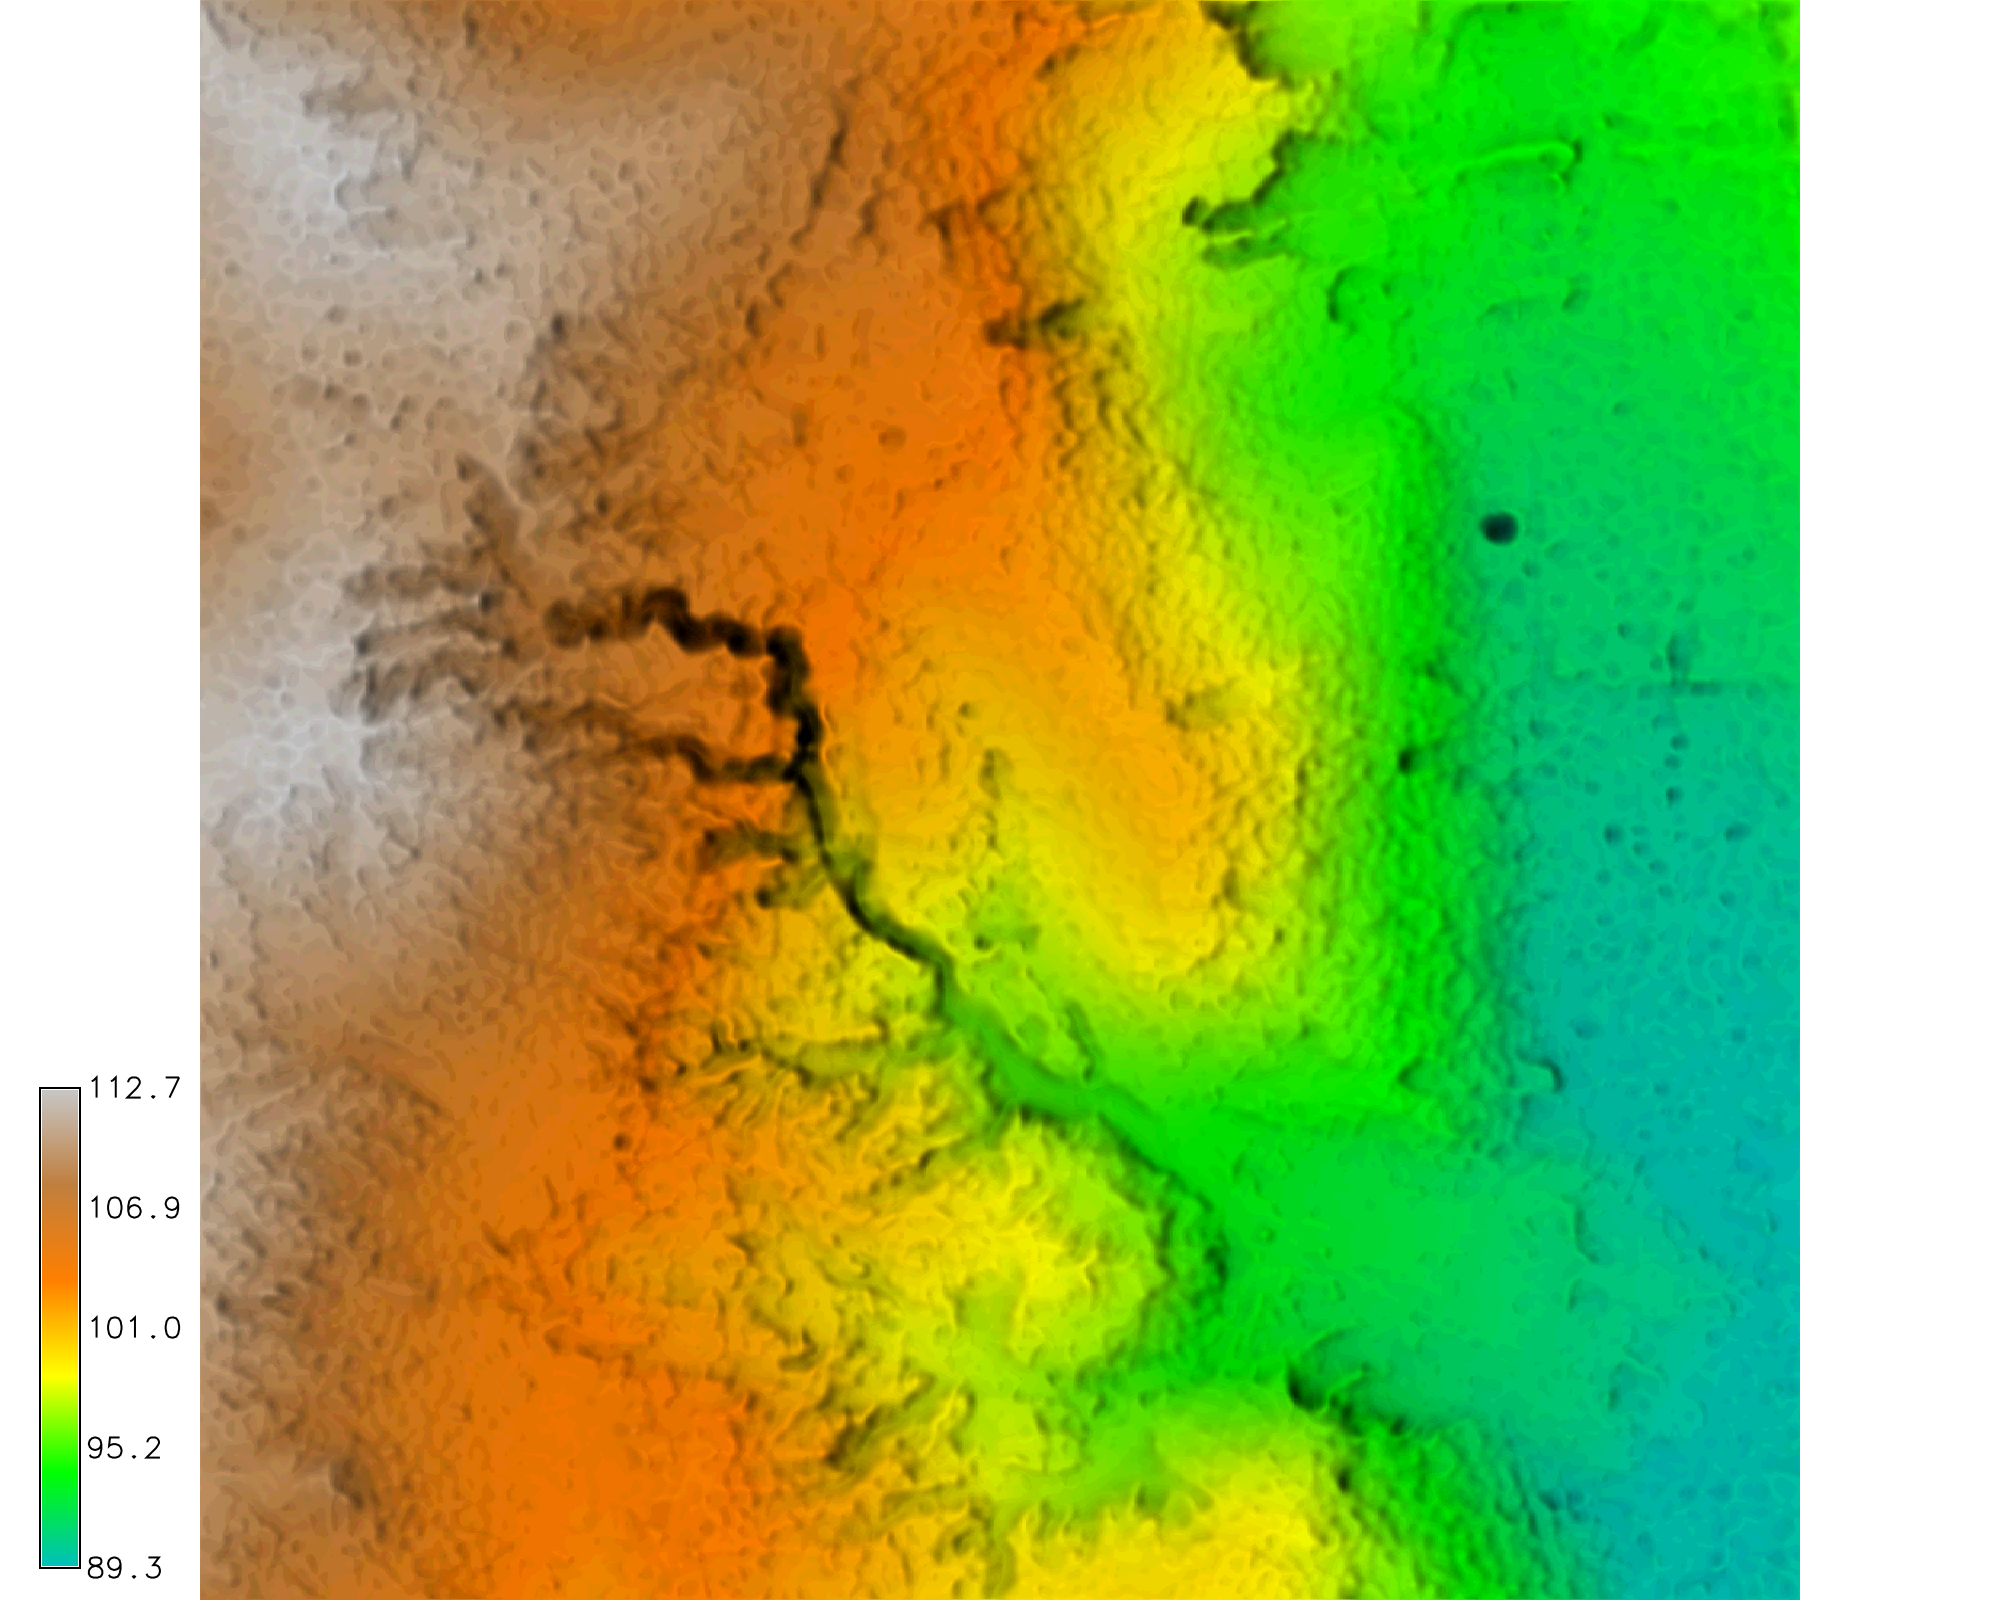
\includegraphics[height=75mm]{../../images/sample_data/elevation_2012.png}} & 
\multicolumn{1}{c}{\begin{overpic}[height=75mm]{../../images/ss_erdep/shaded_relief.png}
\put(0,0){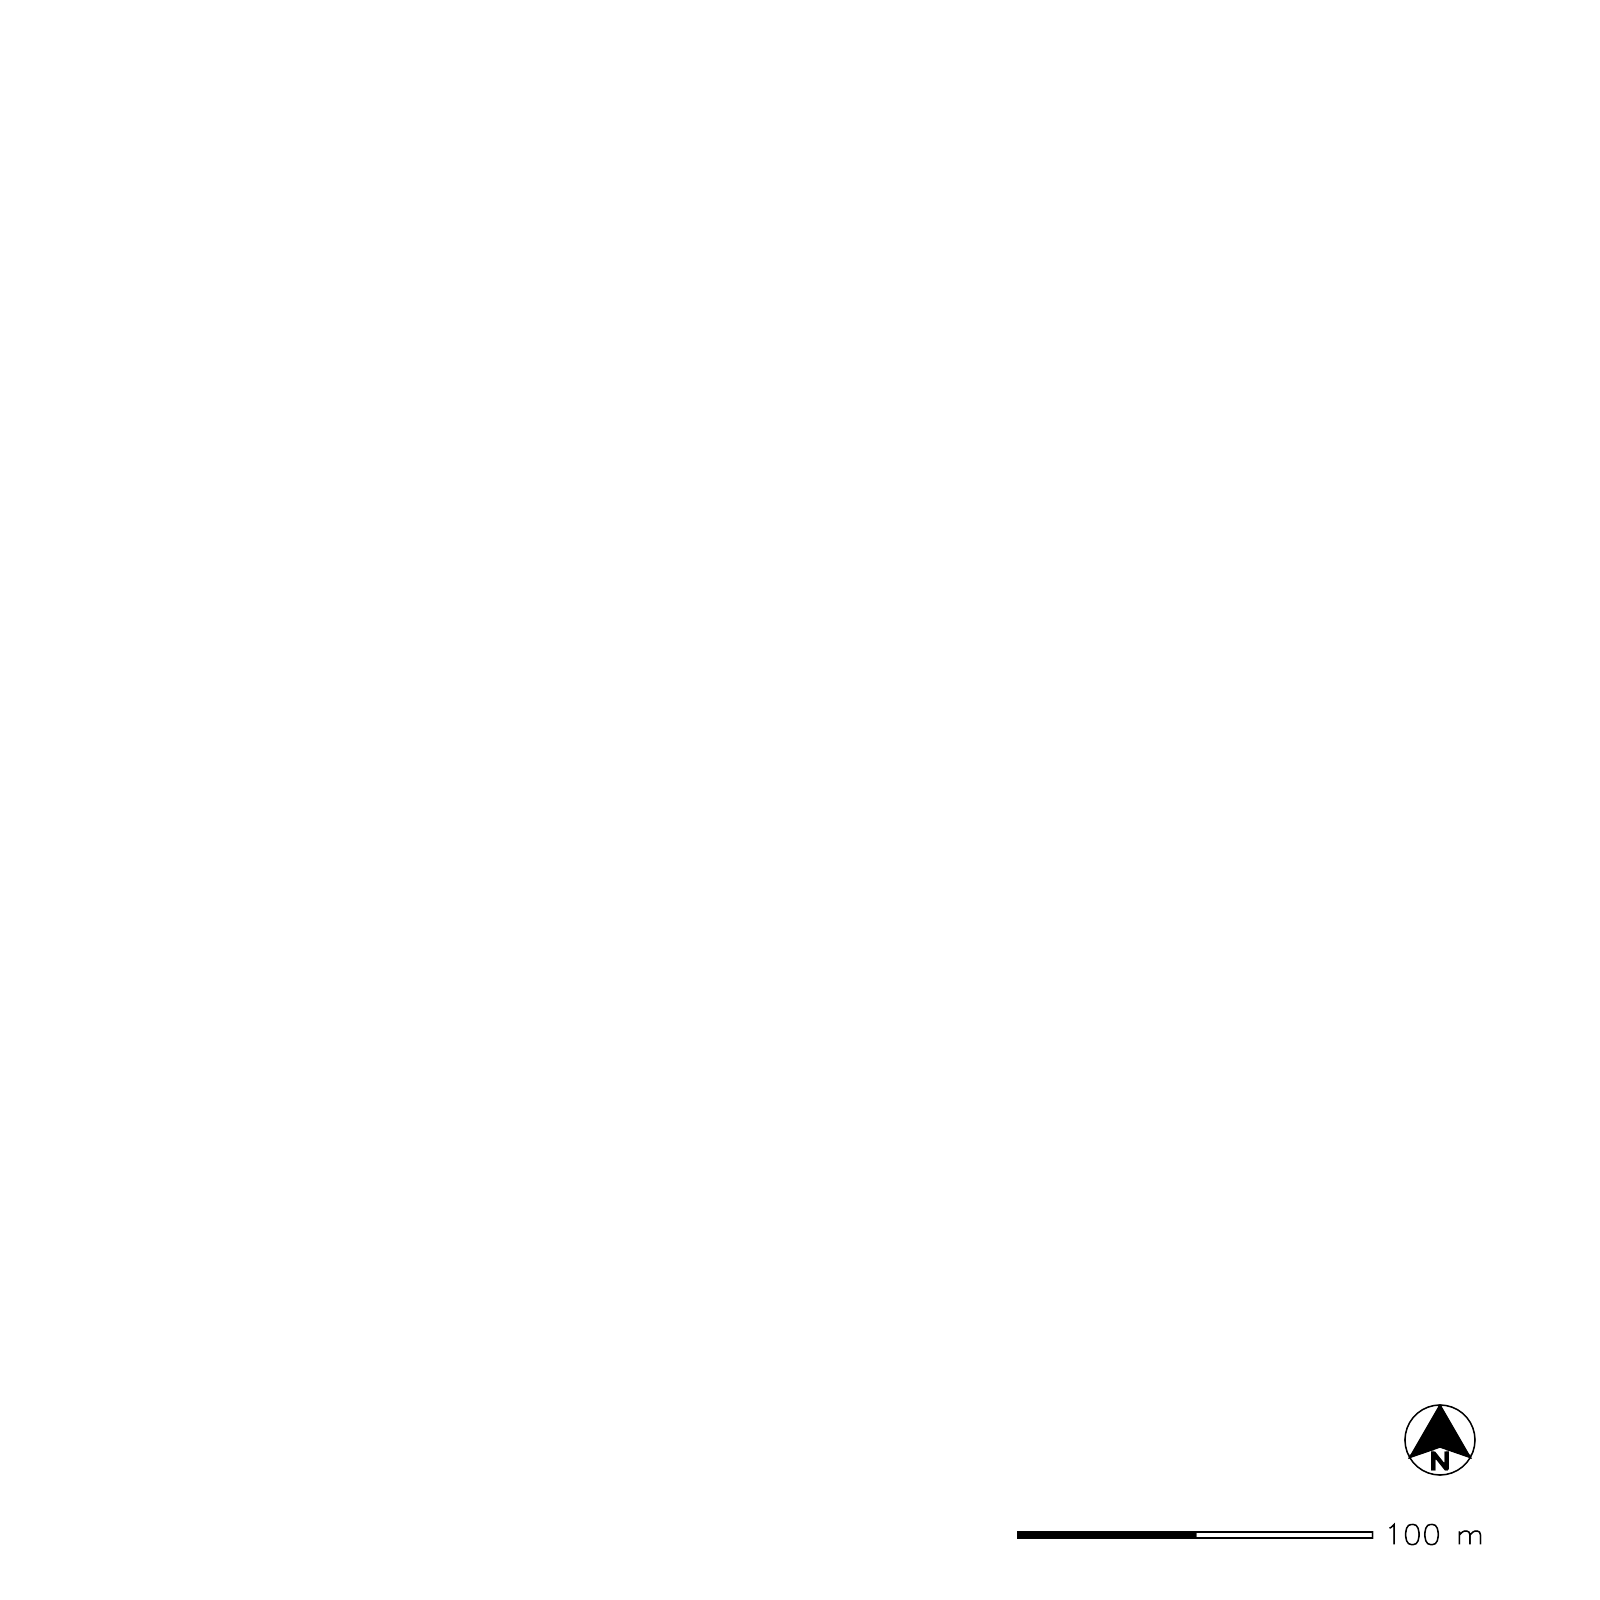
\includegraphics[height=75mm]{../../images/sample_data/map_elements.png}}  
\end{overpic}}
\\
%
\multicolumn{1}{c}{a. DEM derived from 2012 airborne lidar survey} & 
\multicolumn{1}{c}{b. DEM generated by a simulation with SIMWE}\\
%
\label{fig:evolution}
\end{tabular}

\end{document}

